\chapter{O-C Diagrams}
\label{Chapter_oc}
\section{O-C Basics}
Observed minus Calculated diagrams is a diagnostic tool and involves the evaluation and interpretation 
of the disagreement between the measure of an observable event and its
predicted value \citep{Sterken2005basic}.
The idea that random processes may be important in determining O-C behaviour is not new, dating back at least to
\cite{Eddington1929}. Before dealing with the consequences for the statistics of
O-C diagrams, it is worthwhile to review possible physical causes of random
cycle-to-cycle period variations \citep{Koen2005stat}.

In astronomy, O-C usually implies a temporal aspect, and is used when
discussing cyclic phenomena where the times of occurrence of a given event is irregular. 
The O-C diagram is then constructed by plotting the quantity O-C as a function of time, the correct interpretation 
of these deviations leads to a better model (and a new O-C diagram).

In variable-star studies, O-C is sometimes expressed as deviations of phase
in the cycle of variability, whereas the time axis is the cycle number (commonly
indicated by $E$). In such studies, the O-C diagram mostly refers to rather
simple C formalisms, viz. linear or quadratic ephemeris formulae, sometimes
combined with a trigonometric periodic term \citep{Sterken2005basic}.

%Period of a recurrent phenomenon is the time interval after which the event 
%goes exactly through a same cycle again. In reality, we deal with cycles, rhythms, waves, and 
%pseudo-periods or characteristic times, in short, with processes that repeat themselves
%in a more or less regular way.

We are dealing with processes that repeat themselves in a more or less regular way.
Any attempt to construct a reliable O-C diagram will fail if a wrong
value of period $P$ is used. But it is not always easy to derive a period from the observational data: 
$P$ is not directly observable, it follows from the
determination of at least two moments of time of the same reference phase (epochs). 
The observation of two such epochs $T_{1}$ and $T_{2}$ immediately provide us an upper limit for $P$. 
When more than two such times are available, the period can be derived by a least-squares solution of a set of
equations
\begin{equation} \label{eq:period}
T_{i} - T_{j} = nP
\end{equation}
where $n$ is an integer, commonly called the cycle number $E$(epoch).

Phase is a position on the cycle of variation, a convenient periodic measure of
elapsed time: $\varphi (t)$ is the fraction of $P$ that elapsed since the occurrence of the
reference time $T_{0}$ and is given by

\begin{equation} \label{eq:phase}
\varphi = \frac{T-T_{0}}{P} ~\bmod~ 1
\end{equation}

The most common approach to the O-C procedure is the one in which one reference 
phase is selected, and where the timings of this reference phase are studied
and interpreted.
Several methods exist to determine the reference phase in a variability curve. 
This methods are discussed in Chapter \ref{Chapter_minima_det}.

\section{Constant and Variable Period}
If $P$ is constant and if its value is known, equation (\ref{eq:period}) leads to

%\begin{equation} \label{eq:Tmin}
%T_{max} = T_{0} + P E
%\end{equation}
%or,
\begin{equation} \label{eq:Tmin2}
T_{min} = T_{0} + P E
\end{equation}
where $T_{min}$ is the time of minimum light, $T_{0}$
is the zero epoch and $E$ is the number of cycles elapsed since the zero epoch. $T_{0}$ and
$P$ are obtained through a least-squares solution. The longer the time interval (in
cycles) over which the data have been collected, the higher will be the accuracy
of the solution for $P$: the uncertainty in $P$ is inversionally proportional to the
number of cycles, and proportional to the r.m.s. scatter of the data.

It is certainly not a trivial task to conclude from experimental data that a
significant period change has occurred. In principle, changes of period could
be described by any mathematical formula expressing $P$ as a function of time.
Thus, the time of epoch $T_{m}$ is

\begin{equation} \label{eq:P_var}
T_{m} = T_{0} + \int P(t)dt   ~~~~~\mathrm{or}~~~~~   T_{m} = T_{0} + \int P(E)dE
\end{equation}

In most cases, relation (\ref{eq:P_var}) is restricted to linear variations, cyclic variations, or
a combination of both of them.

Many causes can lead to period variations.
%the reference phase is seen systematically earlier (negative O-C) or later (positive O-C), 
%depending whether eclipsing variable is nearer or further from the observer. 
%Such meandering of the reference phase will result in a cyclic O-C diagram. 
%Apsidal motion in an elliptical orbit can re-orient the orbit with
%respect to the observer and cause an effect similar to the previous case. 
Transfer of matter (between stars in a multiple system) or mass ejection (from a system)
can provoke period changes. Periodic variations of O-C can indicate presents of other body in binary system.

If period changes linear with time, we will write $P$ as $P = a+bt$, where $t$ is the time, and $a,~b$ are constants.
Let $P_{0}$ be the period at $t=0$ and $\bar{P}$ is the average period over the whole time of observations, then

\begin{equation} \label{eq:P_lin_P}
P = a + b \bar{P}E
\end{equation} 
and
\begin{equation} \label{eq:P_lin_Pmid}
\bar{P} = a + \frac{1}{2}bt
\end{equation}  
so
\begin{equation} \label{eq:P_lin_Tm}
T_{m} = T_{0} + aE + \frac{1}{2}b \bar{P}E^{2}
\end{equation} 
with
\begin{equation} \label{eq:P_lin_add}
P_{0} = a,  ~~~~  \frac{dP}{dE} = b\bar{P},   ~~~~   \frac{dP}{dt} = b
\end{equation} 
expected time
\begin{equation} \label{eq:P_lin_Tm_res}
T_{m} = T_{0} + P_{0}E + \frac{1}{2} \frac{dP}{dt} \bar{P}E^{2}
\end{equation} 

\begin{equation} \label{eq:P_lin_OC_res}
O-C = \frac{1}{2} \frac{dP}{dt} \bar{P}E^{2}
\end{equation} 

%Equation (\ref{eq:P_lin_Tm}) is the most-frequently applied equation in O-C discussions. 
%Unfortunately, it is often misunderstood. Worse even, the factor $1/2$ is occasionally
%forgotten. The numerical value of $\frac{dP}{dt}$ is obtained through a quadratic fit, which
%also yields $P_{0}$.

When we now look at the O-C diagram for BW Vul in Fig.\ref{fig_oc}, we see that its
shape suggests a possible parabolic form, which seems to stand for a linear period
change. The least-squares parabolic fit to equation (\ref{eq:P_lin_Tm}) yields $P_{0} = 0.2010274$
and $\frac{dP}{dt}= 1.8 \cdot 10^{−10}$ days per cycle, or $~9.1 \cdot 10^{−10}$ day per day.

\begin{figure}[!ht]
\vspace{0cm}
\centerline{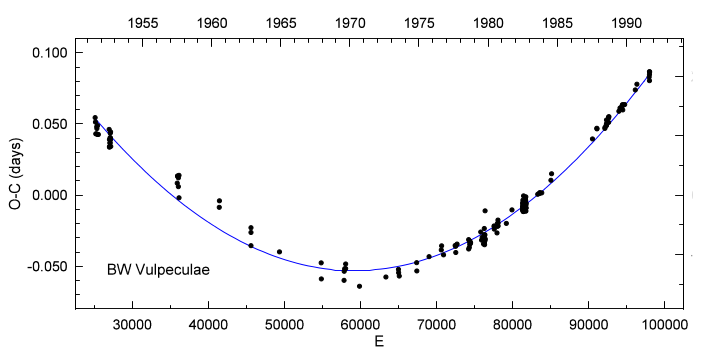
\includegraphics[width=0.65\textwidth]{oc_example.png}}
\caption{O-C diagram of some $T_{min}$ of BW Vul with best fit parabola. \citep{Sterken2005basic}}
\label{fig_oc}
\end{figure}

\begin{figure}[!ht]
\vspace{0cm}
\centerline{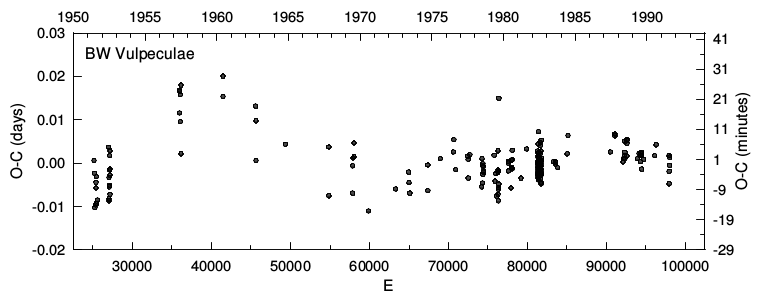
\includegraphics[width=0.65\textwidth]{oc_example_2.png}}
\caption{Differential O-C diagram after prewhitening with the fitted parabola. \citep{Sterken2005basic}}
\label{fig_oc2}
\end{figure}

When looking at Fig.\ref{fig_oc}, one notices that there are stretches of the O-C parabolic
fit where the data at one time are systematically above the fitted curve, and at
other times remain below the curve. Figure \ref{fig_oc2} shows the differences that were
obtained by removing the parabolic trend, and shows wave shape with
variable amplitude \citep{Sterken2005basic}. Such a trend, in particular when it repeats itself, 
can indicate presence of other body in binary system. 
In such case, O-C can be fitted with additional term corresponding to 3rd body orbit parameters:  

\begin{equation} \label{eq:P_lin_OC_sin}
T_{m} = T_{0} + P_{0}E + \frac{1}{2} \frac{dP}{dt} \bar{P}E^{2} +
\dfrac{a_{12}\sin i}{c}   \left[  \dfrac{1-e^2}{1+e \cos\nu}   \sin(\nu + \omega)  + e \sin \omega  \right]
\end{equation} 
 

%\begin{equation} \label{eq:P_lin_OC_sin}
%T_{m} = T_{0} + P_{0}E + \frac{1}{2} \frac{dP}{dt} \bar{P}E^{2} + A\sin(2\frac{\pi}{\Pi}E+\phi)
%\end{equation} 
%
%\begin{equation}\label{eq:4_mmm}
%T_{min} = JD_{0}+P \times E + Q \times E^2 + \dfrac{a_{12}\sin i}{c}   \left[  \dfrac{1-e^2}{1+e \cos\nu}   \sin(\nu + \omega)  + e \sin \omega  \right] 
%\end{equation}
where $a_{12} \sin i$ is the projected semi-major axis, $e$ is the eccentricity,
$\omega$ is the longitude of the periastron, $\nu$ is the true anomaly of the EB orbit around the common centre of the mass of
the whole system and $c$ is the velocity of light \citep{irwin1959}.
